\documentclass[a5paper, DIV=18, 12pt]{scrartcl}
%\usepackage{balloonspectacular}
\usepackage{multicol}
\setlength\columnsep{0.0cm}
\usepackage{enumitem}
\usepackage[margin=0.925cm]{geometry}


\usepackage{fontspec}
\usepackage[dvipsnames]{xcolor}
\usepackage{tikz}
\setmainfont[Scale=1.0]{URWClassico}
\usepackage{eso-pic}

\setkomafont{section}{\setmainfont[Scale=1.125]{Londrina-Solid}\LARGE}
\setkomafont{subsection}{\setmainfont{Fredoka-Bold}\Large}
\setkomafont{subsubsection}{\setmainfont{Fredoka-Bold}\large}

% Adjust spacing before and after section headings
\RedeclareSectionCommand[
  runin=false,
  beforeskip=1.5\baselineskip,
  afterskip=0.5\baselineskip
]{section}

% Adjust spacing before and after subsection headings
\RedeclareSectionCommand[
  runin=false,
  beforeskip=1.0\baselineskip,
  afterskip=0.25\baselineskip
]{subsection}

% Adjust spacing before and after subsubsection headings
\RedeclareSectionCommand[
  runin=false,
  beforeskip=1.0\baselineskip,
  afterskip=0.25\baselineskip
]{subsubsection}

\definecolor{eruption_purple}{HTML}{513c3c}
\definecolor{eruption_pink}{HTML}{ff7280}
\definecolor{eruption_orange}{HTML}{fe6737}

%\pagecolor{eruption_orange!85}
\pagestyle{empty}
\begin{document}
\AddToShipoutPictureBG{
\begin{tikzpicture}[remember picture, overlay]
	\node[opacity=0.25] () at (current page.center) {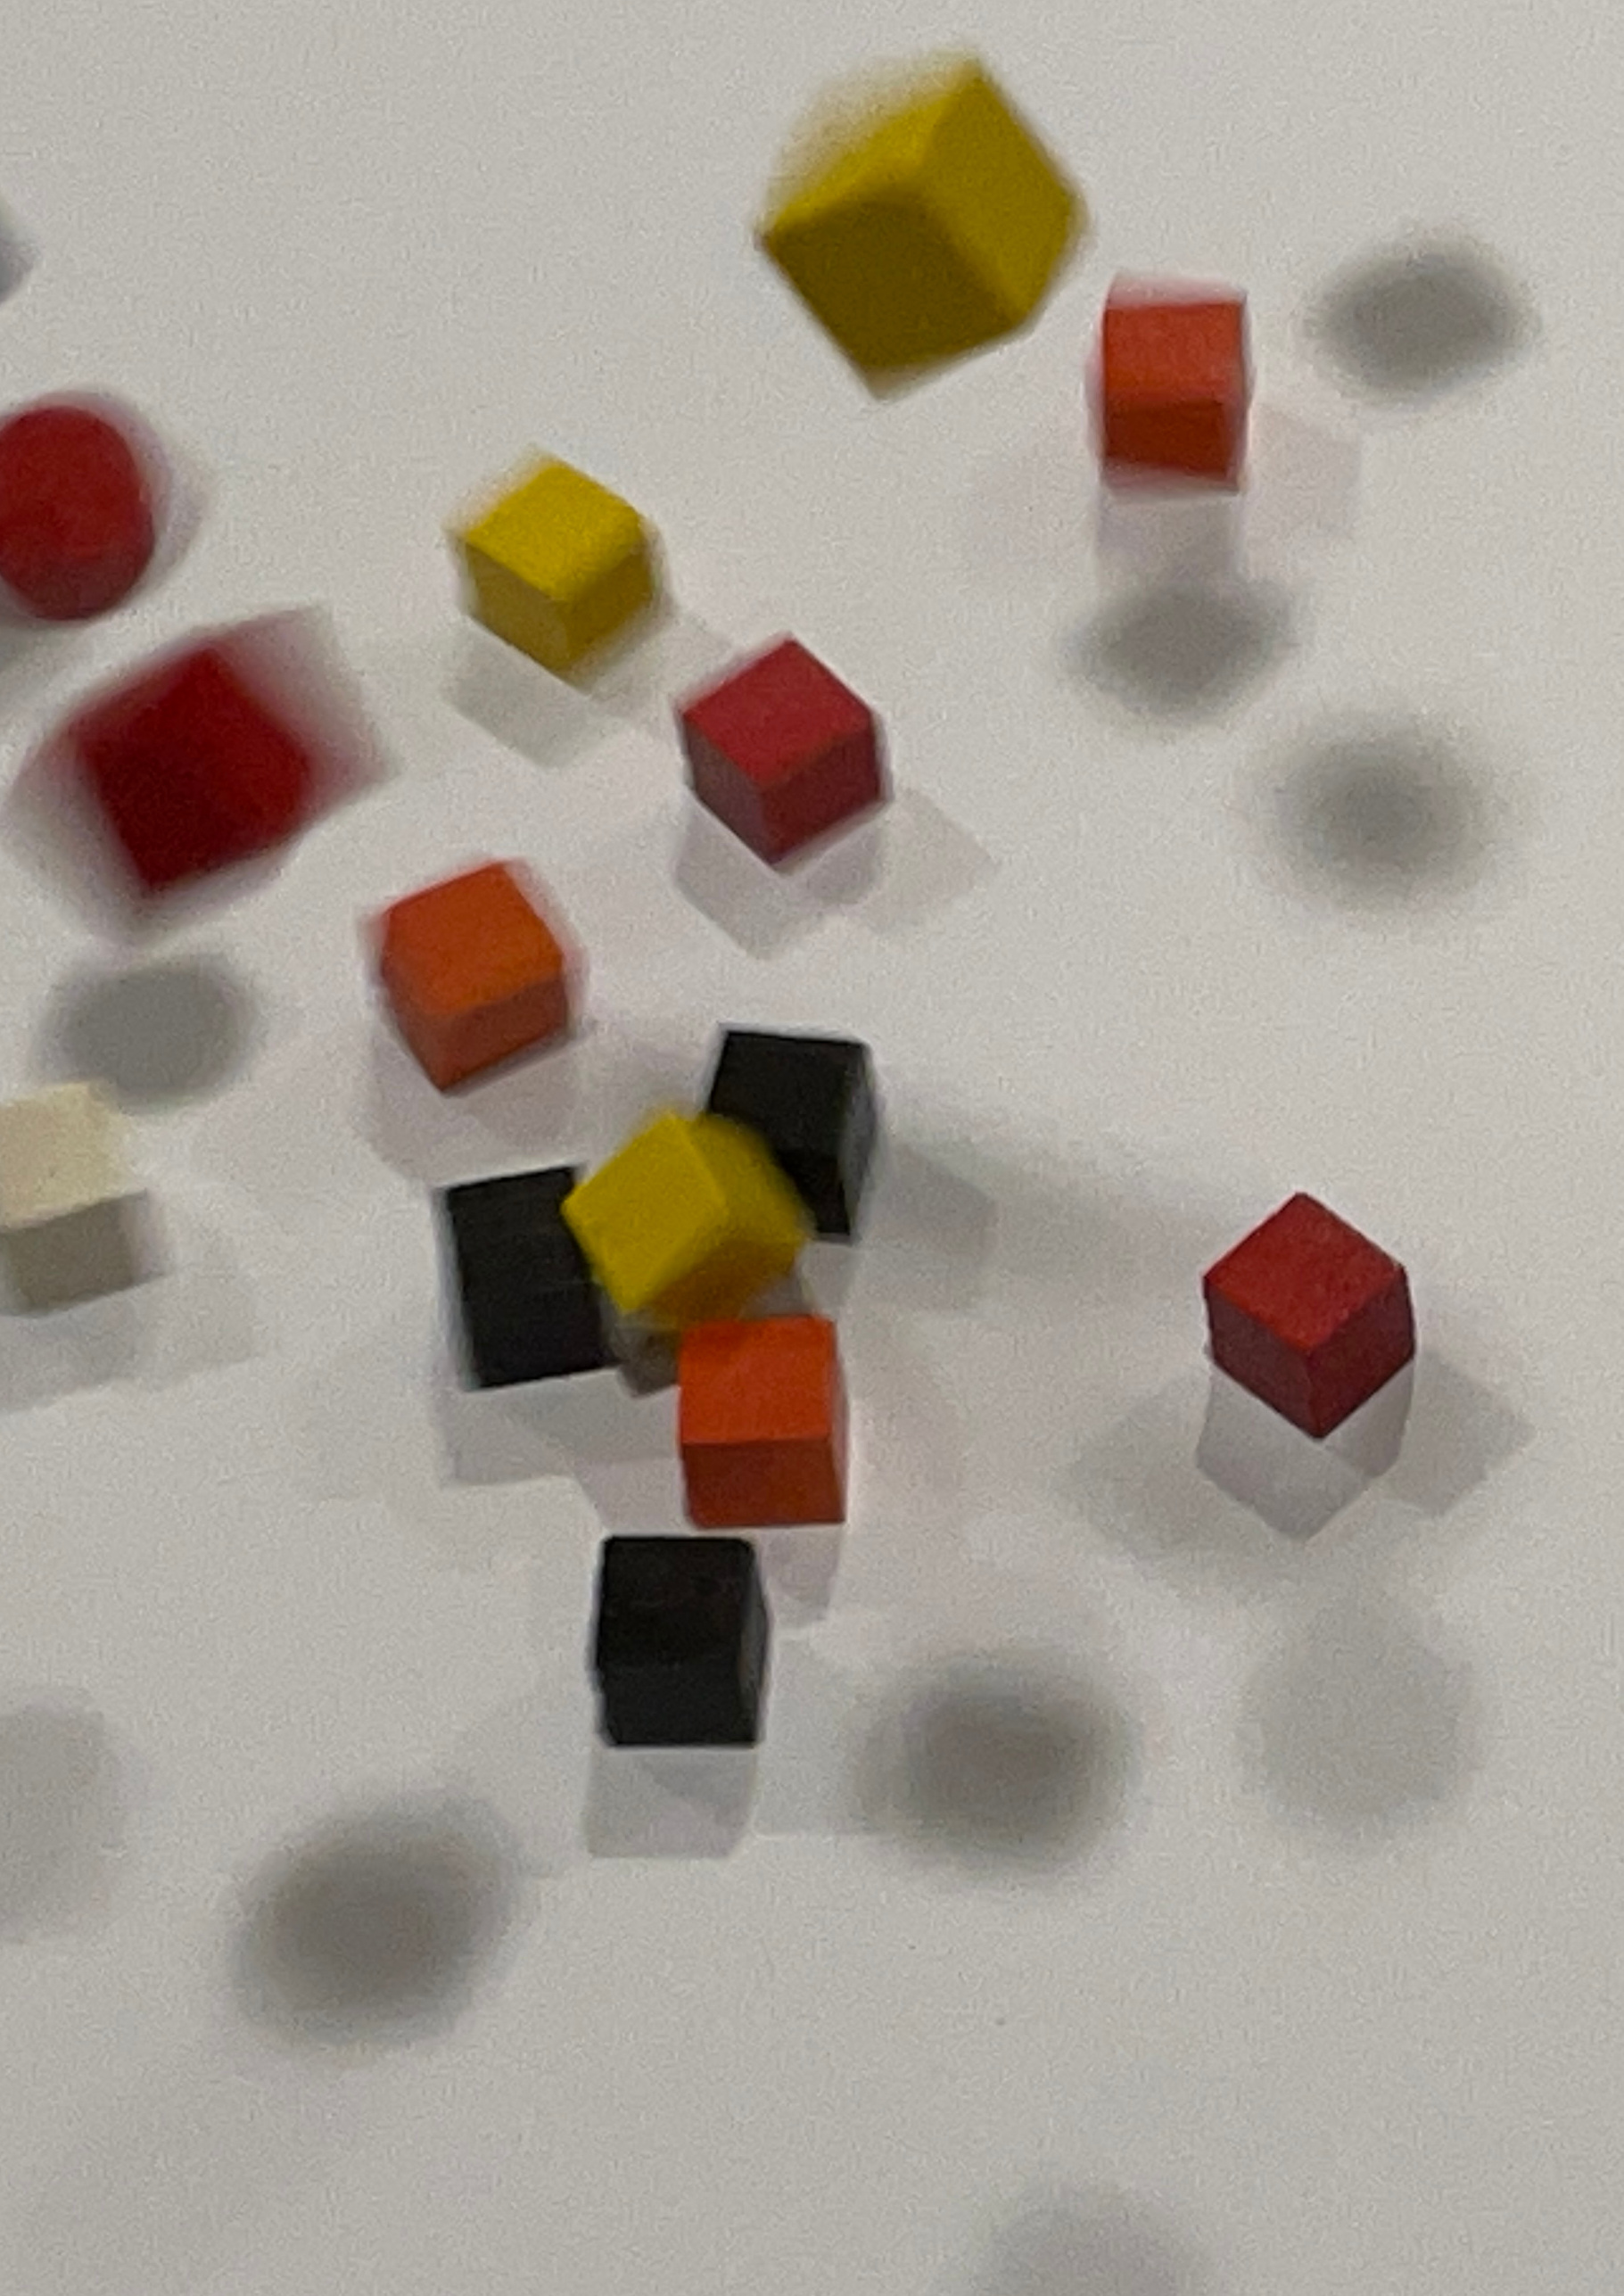
\includegraphics[width=\pagewidth, height=\pageheight]{Images/eruption_background3.jpg}};
\end{tikzpicture}
}

\enlargethispage{1\baselineskip}
%\begin{tikzpicture}
%%\path[draw, red] (-74.25mm, -105mm) -- (74.25mm,105mm);
%\node[inner sep=0mm] at (0,80mm) {{\setmainfont[Scale=3.0]{Oi}\Huge Aloft}};
%\node[inner sep=0mm] at (0,60mm) {{\setmainfont[Scale=1.25]{Playball}\Huge Designed by Michael Purcell}};
%\node[inner sep=0mm] at (0, 40mm) {This is a test};
%\end{tikzpicture}
\vspace{-1ex}
\begin{center}
%\setmainfont[Scale=4.75]{Earthquake MF}
%\colorbox{eruption_pink}{\textcolor{eruption_purple}{\phantom{.}\hfill{}ERUPTION\hfill\phantom{.}}}
%\includegraphics[width=\textwidth]{Images/aloft_banner.png}
\setmainfont[Scale=5.455]{Earthquake MF}
\textcolor{eruption_purple}{ERUPTION}
\end{center}
\vspace{-0.0ex}

\includegraphics[scale=0.125]{Images/Icons/player_count_icon_purple.png} {\setmainfont[Scale=1.25]{Londrina-Solid}\Huge \raisebox{6.55pt}{\textcolor{eruption_purple}{:\ 2-6}}} \hfill 
\includegraphics[scale=0.125]{Images/Icons/player_age_icon_purple.png} {\setmainfont[Scale=1.125]{Londrina-Solid}\Huge \raisebox{6.55pt}{\textcolor{eruption_purple}{:\ 12+}}}\hfill 
\includegraphics[scale=0.125]{Images/Icons/playtime_icon_purple.png} {\setmainfont[Scale=1.125]{Londrina-Solid}\Huge \raisebox{6.55pt}{\textcolor{eruption_purple}{:\ 10-15}}}
\vspace{-0.25ex}
\flushleft
Eruption is a dexterity game about volcanoes. During the game, pressure will mount as you fill rubber-band volcanoes with wooden cubes. Be careful! If the pressure gets too high, a volcano will erupt and spray its cubes all over the table. If that happens on your turn, you will be eliminated from the game. 
\flushleft
\vspace{-0ex}
\begin{multicols}{2}
\section*{\textcolor{eruption_purple}{Features}}
%Eruption is an engaging and\\challenging dexterity game that\\comes in a small package.
%
%\vspace{1.25ex}
%
%It uses only readily-available\\components to create a unique\\game experience for players.
\begin{itemize}[leftmargin=*, nosep]
\item Compact dexterity game
\vspace{0.9ex}
\item Engaging and challenging
\vspace{0.9ex}
\item Uses standard components
\vspace{0.9ex}
\item Unique game experience
\vspace{0.9ex}
\item Attention-grabbing gameplay
\end{itemize}

\section*{\textcolor{eruption_purple}{Gameplay}}
Start by placing the rubber-band volcanoes flat on the table.

\vspace{1.25ex}

On your turn, place a cube into\\a volcano without letting any of\\the existing cubes escape.

\vspace{1.25ex}

As the rubber bands stretch, pressure builds and the task becomes more difficult.

\vspace{3.0ex}

\textbf{Design:} Michael Purcell

%\vfill\null\columnbreak

\section*{\textcolor{eruption_purple}{Components}}
\begin{itemize}[leftmargin=*, nosep]
	\item 175 wooden cubes (8mm)
	\begin{itemize}[leftmargin=*, nosep]
	\vspace{0.9ex}
	  \item 120 lava-colored cubes
	  \vspace{0.9ex}
	  \item 50 black cubes
	  \vspace{0.9ex}
	  \item 5 white cubes
	\end{itemize}
	\vspace{0.9ex}
	\item 5 rubber bands (size \#31)
\end{itemize}

\vspace{6ex}

%\quad 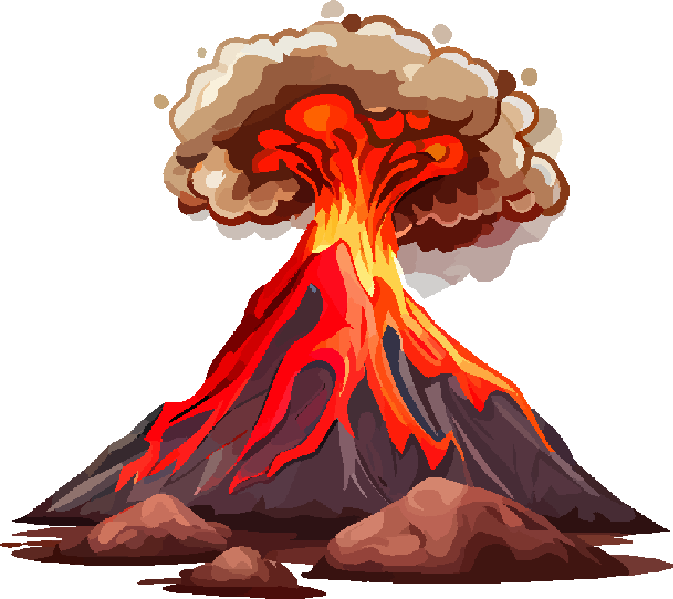
\includegraphics[width=0.7\columnwidth]{Images/one_volcano.png}
\qquad 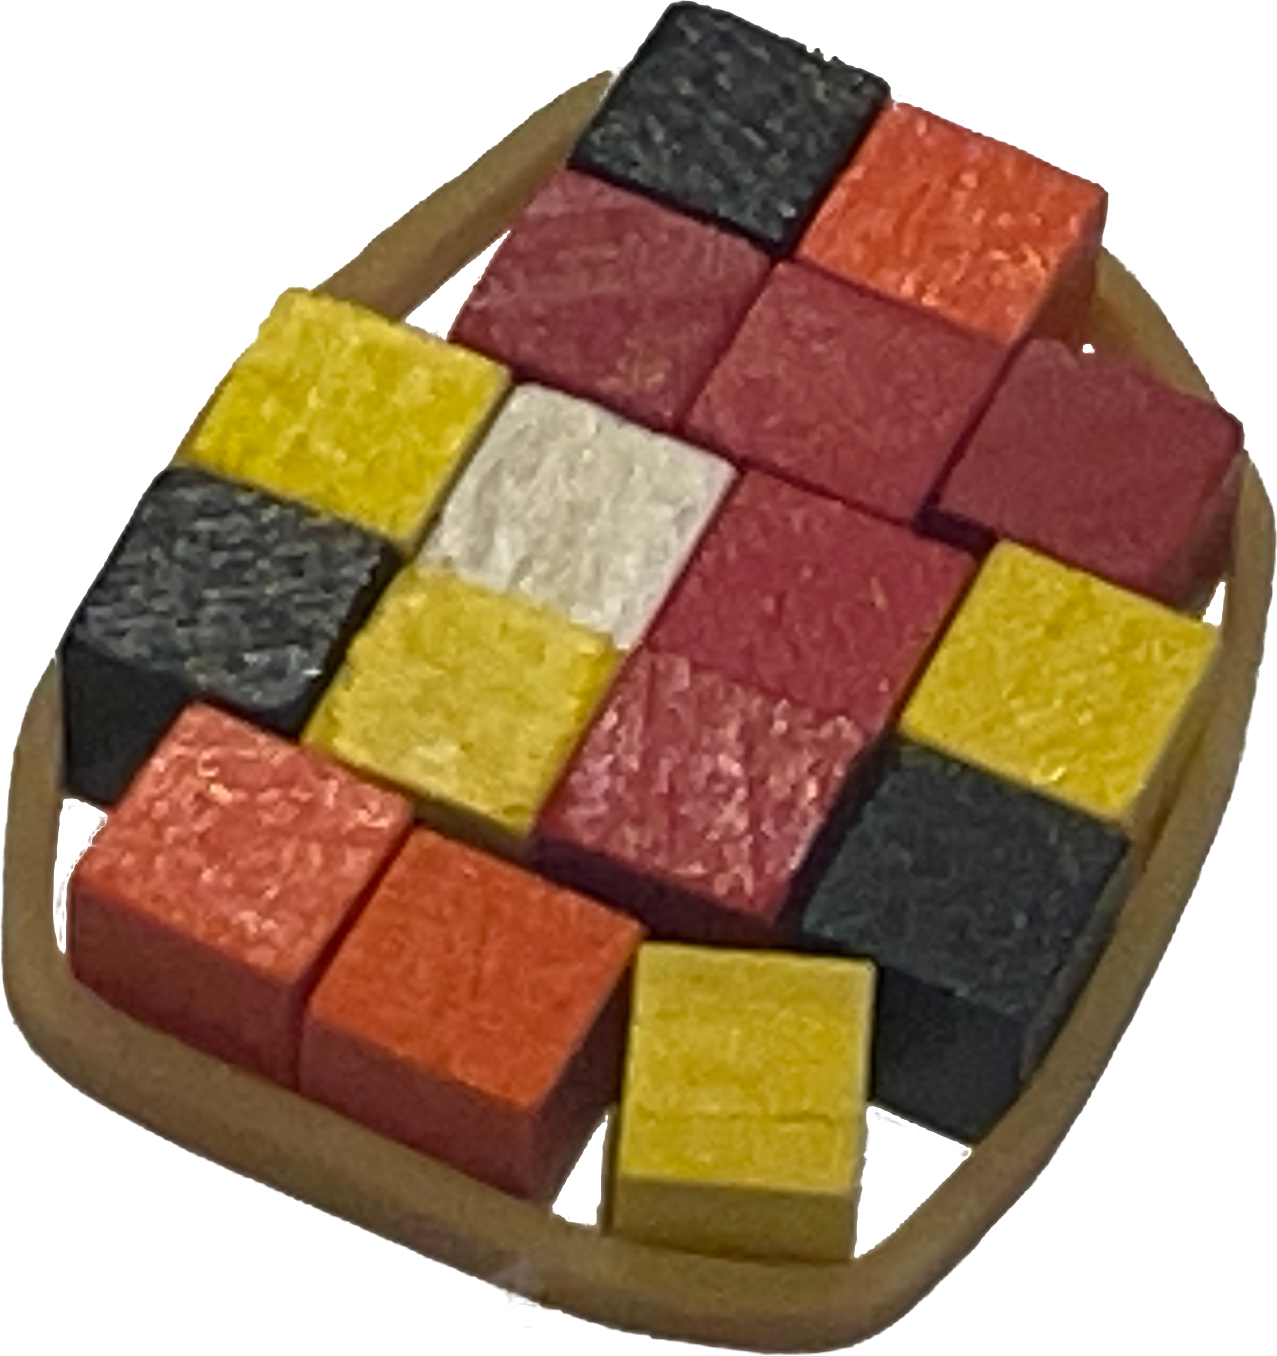
\includegraphics[width=0.55\columnwidth]{Images/eruption1.png}

\vspace{2ex}
Dramatic eruptions ensure that\\every game ends with a bang!  

%\vspace{3.25ex}
\vfill{}

\textbf{Contact:} ttkttkt@gmail.com
%{\setmainfont[Scale=1.125]{Fredoka-Bold}\LARGE \hfill \textcolor{SunriseBlue}{Up, Up, and Away!}}
\end{multicols}
%\begin{center}
%%\includegraphics[width=\textwidth]{Images/sell_sheet_diagram.png}
%\end{center}
%\vspace{-7ex}
%%\hrule
%%\vspace{2ex}
%\textbf{Design:} Michael Purcell \hfill \textbf{Contact:} ttkttkt@gmail.com
\end{document}